\documentclass{jknotes}
\usepackage{../joshkirklin}

\setmathfont{Latin Modern Math}
\setmathfont{GFS NeoHellenic Math}[range=bfsfup/{greek,Greek}->it]
\setmathfont{GFS NeoHellenic Math}[range=sfup/{latin,Latin}->it]

\usetikzlibrary{shapes.misc}

\tikzset{cross/.style={cross out, draw=black, minimum
size=2*(#1-\pgflinewidth), inner sep=0pt, outer sep=0pt}}
%default radius will be 1pt. 

\newcommand{\myol}[2][3]{{}\mkern#1mu\overline{\mkern-#1mu#2}}

\begin{document}

\institution{Cambridge Part III Maths}
\title{Fluid Dynamics of Environment}
\lecturer{Dr. Stuart Dalziel}
\notetaker{Charles Powell}
\date{Lent 2020}

\maketitle
\suggestionsspiel
\tableofcontents

\lecture{22/01/21}
\section{Internal waves}

\subsection{Intuitive version}

\begin{center}
	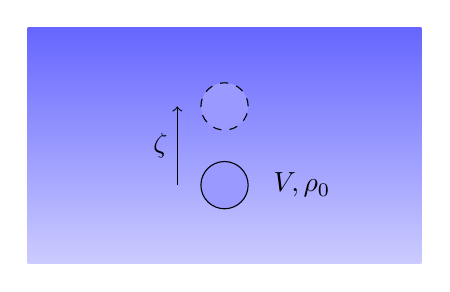
\begin{tikzpicture}
		\draw[draw=none,top color = blue!60, bottom color = blue!20] (0,0) rectangle (5, 3);
		\draw[fill=blue!40] (2.5, 1) circle (0.3);
		\draw (3, 1) node[right] {$V, \rho_0$};
		\draw[dashed,fill=blue!40] (2.5, 2) circle (0.3);
		\draw[->] (1.9, 1) -- (1.9, 2) node[midway,left] {$\zeta$};
	\end{tikzpicture}
\end{center}
Consider a fluid parcel of volume $V$ and density $\rho_0$ in a fluid with
density profile $\hat{\rho}(z)$.  Suppose the parcel is moved upwards by
$\zeta$. The parcel experiences a \emph{buoyancy force} $B = g V \zeta
\frac{\diffd \hat{\rho}}{\diffd z}$. Newton's second law gives
\begin{equation}
	\ddot{\zeta} + \left(-\frac{g}{\rho_0} \frac{\diffd \hat{\rho}}{\diffd
	z}\right) \zeta = 0
\end{equation}
The \emph{buoyancy frequency} (or Brunt-V\"{a}is\"{a}l\"{a} frequency) is
defined as 
\begin{equation}
	N^2 = - \frac{g}{\rho} \frac{\diffd \hat{\rho}}{\diffd z}
\end{equation}
which has general solution
\begin{equation}
	\zeta = A \cos N t + B \sin N t
\end{equation}
If we instead consider a fluid slab inclined at angle $\theta$ with the
vertical rather than a fluid parcel, the slab can fall in its plane much more
easily than in the vertical. Hence in this situation we have
\begin{equation}
	\ddot{\zeta} + N^2 \cos^2\theta \zeta = 0
\end{equation}
The dispersion relation is thus $\omega/N = \cos \theta$.

Now consider a sphere oscillating at frequency $\omega$ in the vertical in a
stratified fluid with density $\rho(z)$. The fluid resonates in bands at angle
$\theta$ satisfying the dispersion relation, provided $\omega < N$.
Intuitively, the group velocity must be out of the beams as energy is radiated
away.
\begin{center}
	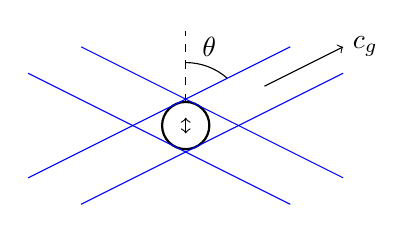
\begin{tikzpicture}
		\draw[thick] (0,0) circle (0.3);
		\draw[<->] (0, 0.1) -- (0, -0.1);
		\draw[blue] (1.328,1) -- (-2, -0.664);
		\draw[blue] (-1.328,-1) -- (2, 0.664);
		\draw[blue] (-1.328,1) -- (2, -0.664);
		\draw[blue] (1.328,-1) -- (-2, 0.664);
		\draw[dashed] (0, 0.3) -- (0, 1.2);
		\draw (0,0.8) arc (90:49:0.8);
		\draw (0.3, 1) node {$\theta$};
		\draw[->] (1, 0.5) -- (2,1) node[right] {$\symbf{c}_g$};
	\end{tikzpicture}
\end{center}

At the leading edge of the rays, baroclinic vorticity is generated by the
movement of fluid of different density to its surroundings. This provides the
mechanism for the instability.

\subsection{Rigorous derivation}
Consider a fluid in which the mean pressure $p_0(z)$ and the mean density
$\rho_0(z)$ are in hydrostatic balance when the fluid is at rest:
\begin{equation}
	\frac{\diffd p_0}{\diffd z} = - \rho_0 g
\end{equation}

Assume that the vertical lengthscale for $\rho_0$ variation is $L$. Motion is
governed by the Navier-Stokes equations \eqref{eq:incomp} and \eqref{eq:ns} with
$\nu = 0$, and mass conservation \eqref{eq:masscons}. 
\begin{align}
	\nabla \cdot \symbf{u} &= 0 \label{eq:incomp} \\
	\rho \frac{\partial \symbf{u}}{\partial t} + \rho
	(\symbf{u}\cdot\nabla)\symbf{u} &= - \nabla p - \rho g \hat{\symbf{z}}
	\label{eq:ns} \\
	\left(\frac{\partial}{\partial t} + \symbf{u}\cdot \nabla \right) \rho = 0
	\label{eq:masscons}
\end{align}

Following the Boussinesq approximation, assume small perturbations to the mean
state: $\rho = \rho_0(z) + \tilde{\rho}$ and $p = p_0(z) + \tilde{p}$ where
$\tilde{p} \ll p_0, \tilde{\rho} \ll \rho_0$. Under this approximation, the
momentum equation \eqref{eq:ns} becomes
\begin{align}
	\frac{\partial \symbf{u}}{\partial t} + (\symbf{u}\cdot\nabla)\symbf{u} 
	&= - \frac{1}{\rho_0}\nabla p - \frac{\rho}{\rho_0} g \hat{\symbf{z}} \\ 
	&= - \frac{1}{\rho_0} \nabla(p + \rho_0 g z) - g' \hat{\symbf{z}}
\end{align}
where $g' = g(\rho-\rho_0)/\rho_0$ is the \emph{reduced gravity}. We now
linearise $\symbf{u}$ about a state of rest, ignoring second order quantities
in the velocity disturbance $\symbf{u}'$. It is now further desirable to split
the disturbance components into $\tilde{\rho} = \hat{\rho} + \rho', \tilde{p}
= \hat{p} + p'$ where $\hat{\rho}, \hat{p}$ are in hydrostatic balance. We
have
\begin{align}
	\nabla \cdot \symbf{u}' &= 0  \\
	\frac{\partial \rho'}{\partial t} + w' \frac{\diffd \hat{\rho}}{\diffd z}
							&= \frac{\partial \rho'}{\partial t} - w' \frac{\rho_0}{g}N^2 
							= 0 \\
	\frac{\partial \symbf{u}'}{\partial t} 
							&= -\frac{1}{\rho_0}\nabla (p_0+\hat{p}) -
							\frac{g\hat{\rho}}{\rho_0}\hat{\symbf{z}} -
							\frac{1}{\rho_0} \nabla p' -
							\frac{g\rho'}{\rho_0}\hat{\symbf{z}}
							\label{eq:idk} 
\end{align}
Hydrostatic balance eliminates the first two RHS terms of the momentum
equation; the
hydrostatic pressure field is 
\begin{equation}
	p_0 + \hat{p} = -\int g \hat{\rho} \, \diffd z
\end{equation}
Finally we have
\begin{equation}
	\frac{\partial \symbf{u}'}{\partial t} = -\frac{1}{\rho_0} \nabla p' -
	\frac{g\rho'}{\rho_0} \hat{\symbf{z}}
\end{equation}
Define buoyancy $b = - g \rho'/\rho_0$. The governing equations are now
\begin{align}
	\frac{\partial b}{\partial t} &= -\frac{1}{\rho_0} \nabla p' + b
	\hat{\symbf{z}} \\
	\frac{\partial \symbf{u}'}{\partial t} &= -\frac{1}{\rho_0} \nabla p' + b
	\hat{\symbf{z}}
\end{align}
To eliminate pressure, we take the curl of the momentum equation to get
\begin{equation}
	\frac{\partial \symbf{\zeta}'}{\partial t} = -\hat{\symbf{z}}\times\nabla
	b
\end{equation}
where $\symbf{\zeta}' = \nabla \times \symbf{u}'$ is the disturbance
vorticity. Using the buoyancy equation we have
\begin{equation}
	\left[ \nabla^2 \frac{\partial^2}{\partial t^2} + N^2 \nabla_H^2\right] w'
	= 0
\end{equation}
where $\nabla_H = (\partial_x,\partial_y)$ is the horizontal gradient
operator. This equation admits plane wave solutions
\begin{equation}
	w'(\symbf{x},t) = \Re\left[ \hat{w}(t) e^{i(k_x x + k_y y - \omega
	t)}\right]
\end{equation}
where $\hat{w}$ satisfies
\begin{equation}
	\frac{\diffd^2 \hat{w}}{\diffd z^2} + (k_x^2 + k_y^2)(\frac{N^2}{\omega^2}
	- 1) \hat{w} = 0
\end{equation}
which has general solution
\begin{align}
	\hat{w} &= \Re\left[ A e^{-inz} + Be^{inz}\right] \\
	n^2 &= (k_x^2 + k_y^2)(\frac{N^2}{\omega^2} - 1)
\end{align}
If $\omega > N$, $n$ is imaginary and, defining $\gamma =
\sqrt{1-N^2/\omega^2}$, we have
\begin{equation}
	w' = (A e^{-\gamma k z} + B e^{\gamma kz}) e^{i(k_x x + k_y y - \omega
	t)}
\end{equation}
When $N = 0$, we get potential flow. If $0 < N < \omega$ then we have rescaled
potential flow, with scaling $\gamma$. If $\omega < N$ then $n$ is real and
solutions are oscillatory with
\begin{equation}
	n^2 = k z^2 = (k_x^2 + k_y^2)(\frac{N^2}{\omega^2} - 1)
\end{equation}
The wavenumber vector is $\symbf{k} = (k_x, k_y, k_z) = (k,l,m)$. Hence
\begin{equation}
	\frac{\omega^2}{N^2} = \frac{k_x^2 + k_y^2}{k_x^2+k_y^2+k_z^2} = 1 -
	\frac{k_z^2}{\abs{\symbf{k}}^2} = \cos^2 \theta
\end{equation}
where $\theta$ is the angle between $\symbf{k}$ and the horizontal plane. Note
that $N$ is assumed constant.

\begin{center}
	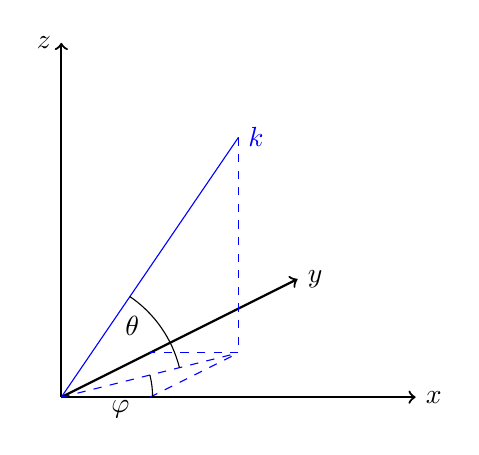
\begin{tikzpicture}[scale=1.5]
		\draw[thick,->] (0,0) -- (3, 0) node[right] {$x$};
		\draw[thick,->] (0,0) -- (0, 3) node[left] {$z$};
		\draw[thick,->] (0,0) -- (2, 1) node [right] {$y$};
		\draw[blue] (0,0) -- (1.5, 2.2) node [right] {$\symbf{k}$};
		\draw[blue,dashed] (1.5, 2.2) -- (1.5, 0.375);
		\draw[blue,dashed] (0,0) -- (1.5, 0.375);
		\draw[blue,dashed] (0.75,0) -- (1.5, 0.375);
		\draw[blue,dashed] (1.5, 0.375) -- (0.75,0.375);
		\draw (1,0.25) arc (14:55.7:1.03);
		\draw (0.75,0.1875) arc (14:0:0.77);
		\draw (0.5, -0.1) node {$\varphi$};
		\draw (0.6, 0.6) node {$\theta$};
	\end{tikzpicture}
\end{center}

We will use $\theta$ as the angle between the horizontal plane and
$\symbf{k}$, hence $\omega/N = \cos \theta$. Some authors use the polar
inclination angle between $\hat{\symbf{z}}$ and $\symbf{k}$, in which case
$\omega/N = \sin\theta$. The azimuthal angle between the $x$ axis and the
projection of $\symbf{k}$ onto the horizontal plane is denoted by $\varphi$.
We will also assume $\omega \ge 0$ going forward. The wavevector takes the
form
\begin{equation}
	\symbf{k} = \abs{\symbf{k}} \begin{pmatrix} \cos\varphi\cos\theta \\
	\sin\varphi\cos\theta \\ \sin \theta \end{pmatrix}
\end{equation}

The \emph{phase} of the wave is defined to be $\phi = \symbf{k}\cdot\symbf{x}
- \omega t$. Note the following:
\begin{align}
	e^{i\phi} &= e^{i(\symbf{k}\cdot\symbf{x}-\omega t)} \\
	\Re\left[ e^{i\phi}\right] &= \Re\left[ e^{-i\phi}\right] \\
	\Re\left[ \tilde{\eta}e^{i\phi}\right] &= \Re\left[\tilde{\eta}^*
	e^{-i\phi}\right]
\end{align}

We will focus on 2D waves. By suitable choice of coordinate system, 3D waves
can be reduced to 2D. In the (x,z) plane, from $\nabla \cdot \symbf{u} = 0$
and assuming $w(\symbf{x},t) = \tilde{w}e^{i\phi}$ with $\tilde{w} \in
\mathbb{C}$ we have
\begin{equation}
	u = \int -\frac{\partial w}{\partial z} \, \diffd x = -\frac{m}{k}
	\tilde{w}e^{i\phi} = - \tan \theta \tilde{w} e^{i\phi}
\end{equation}
\begin{center}
	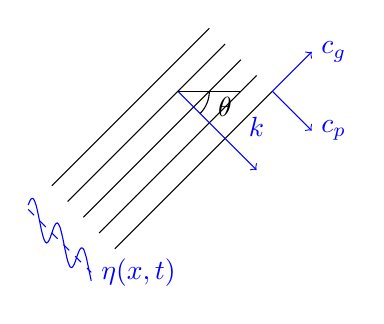
\begin{tikzpicture}
		\draw (0,0) -- ++ (2,2);
		\draw (0.2, -0.2) -- ++(2,2);
		\draw (0.4, -0.4) -- ++(2,2);
		\draw (0.6, -0.6) -- ++(2,2);
		\draw (0.8, -0.8) -- ++(2,2);
		\draw[blue,->] (1.6, 1.2) --++(1,-1);
		\draw[blue,dashed] (-0.3, -0.3) -- ++ (0.8, -0.8);
		\draw[smooth,blue] plot[domain=-0.3:0.5]
		({\x},{0.2*sin(20*deg(\x))-\x-0.6});
		\draw[blue] (1.1, -1.1) node {$\eta(\symbf{x},t)$};
		\draw[blue] (2.6, 0.75) node {$\symbf{k}$};
		\draw[blue,->] (2.8, 1.2) -- ++(0.5, -0.5) node [right] {$\symbf{c}_p$};
		\draw[blue,->] (2.8, 1.2) -- ++(0.5, 0.5) node [right] {$\symbf{c}_g$};
		\draw (1.6, 1.2) -- (2.4, 1.2);
		\draw (2,1.2) arc (0:-45:0.4);
		\draw (2.2, 1) node {$\theta$};
	\end{tikzpicture}
\end{center}
Denoting the wave displacement by $\eta(\symbf{x},t) = \tilde{\eta}e^{i\phi}$
we have the following:
\begin{align}
	\frac{\partial \eta}{\partial t} &= -i\omega \tilde{\eta} e^{i\phi} \\
	u(\symbf{x},t) &= \tilde{u}e^{i\phi} = -i\omega \sin\theta
	\tilde{\eta}e^{i\phi} \\
	w(\symbf{x},t) &= \tilde{w}e^{i\phi} = i\omega \cos\theta
	\tilde{\eta}e^{i\phi} \\
\end{align}

Using the buoyancy equation $\partial b / \partial t = - w N^2$ we also find
\begin{equation}
	i\omega \tilde{b} = - \tilde{w}N^2 \implies b = - \tilde{\eta}
	\frac{\omega^2}{\cos\theta} e^{i\phi} = - \tilde{\eta}\omega N e^{i\phi}
\end{equation}
Similarly the pressure field follows from the momentum equation
\begin{equation}
	\frac{\partial u}{\partial t} = - \frac{1}{\rho_0} \frac{\partial
	p'}{\partial x} \implies \tilde{p} = i\frac{\omega^2}{k}
	\tilde{\eta}\sin\theta
\end{equation}

\subsection{Wave velocities}
\subsubsection{Phase velocity}
For the phase $\phi =
\symbf{k}\cdot\symbf{x} - \omega t$ we can write
\begin{align}
	\frac{\partial \phi}{\partial x_i} \frac{\partial \phi}{\partial t} -
	\frac{\partial \phi}{\partial t} \frac{\partial \phi}{\partial x_i} &= 0
	\\
	\implies k_i \frac{\partial \phi}{\partial t} + \omega \frac{\partial
\phi}{\partial x_i} &= 0\\
\implies \frac{\partial \phi}{\partial t} + \frac{\omega}{\abs{\symbf{k}}^2}
k_i \frac{\partial \phi}{\partial x_i}
\end{align}
Defining the phase velocity $\symbf{c}_p = \frac{\omega}{\abs{\symbf{k}}^2}
\symbf{k}$ as the velocity at which the phase is advected, we have
\begin{equation}
	\frac{\partial \phi}{\partial t} + (\symbf{c}_p \cdot \nabla) \phi = 0
\end{equation}

For all waves, this is the speed at which wave crests move. For deep water
waves with dispersion relation $\omega = \sqrt{gk}$ we find $c_p =
\sqrt{g/k}$. 

\subsubsection{Group velocity}
By symmetry of partial differentiation, we may write
\begin{align}
	\frac{\partial^2 \phi}{\partial t \partial x_i} - 
	\frac{\partial^2 \phi}{\partial t \partial x_i} &= 0 \\
	\implies \frac{\partial k_i}{\partial t} + \frac{\partial \omega}{\partial
x_i} &= 0 \label{eq:132}
\end{align}
If $\omega = \omega(\symbf{k})$ then from chain rule
\begin{equation}
	\frac{\partial \omega}{\partial x_i} = \frac{\partial \omega}{\partial
	k_j} \frac{\partial k_j}{\partial x_i}
\end{equation}
We also know from definition of phase
\begin{equation}
	\frac{\partial k_j}{\partial x_i} = \frac{\partial}{\partial x_i} \left(
	\frac{\partial \phi}{\partial x_j} \right) = \frac{\partial k_i}{\partial
	x_j}
\end{equation}
Hence  \eqref{eq:132} may be written as
\begin{equation}
	\frac{\partial k_i}{\partial t} + \frac{\partial \omega}{\partial k_j}
	\frac{\partial k_i}{\partial x_j} = 0
\end{equation}
Thus we define the group velocity as the velocity at which the wavevector is
advected, i.e. $\symbf{c}_g = \frac{\partial \omega}{\partial k_i}$ and
\begin{equation}
	\left( \frac{\partial}{\partial t} + \symbf{c}_g \cdot \nabla \right)
	\symbf{k} = 0
\end{equation}
For deep water waves, we thus have $c_g = \sqrt{g/k}/2 = c_p/2$.
\subsubsection{Superposition}
Consider two waves with slightly different wavenumber and frequency
superposed:
\begin{align}
	\eta &= \cos \left( (k+\delta k)x - (\omega+\delta \omega)t\right) + \cos
	\left( (k-\delta k)x - (\omega - \delta\omega)t\right) \\
		 &= 2 \cos \left( \delta k x - \delta \omega t\right) \cos \left( kx -
		 \omega t\right)
\end{align}
This is referred to as \emph{modulation} with $\abs{\delta k} \ll \abs{k},
\abs{\delta \omega} \ll \abs{\omega}$. Equivalently, in the limit as
$\abs{\delta k} \to 0, \abs{\delta \omega} \to 0$, we have
\begin{equation}
	\eta = 2 \cos \left( (x-\frac{\partial \omega}{\partial k} t)\delta
	k\right)
	\cos \left( kx - \omega t \right)
\end{equation}

\begin{center}
	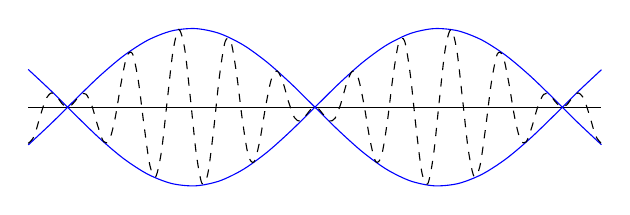
\begin{tikzpicture}
		\draw (-0.5,0) -- (6.78, 0);
		\draw[smooth,blue] plot[domain=-0.5:6.78] ({\x},{sin(deg(\x))});
		\draw[smooth,blue] plot[domain=-0.5:6.78] ({\x},{-sin(deg(\x))});
		\draw[smooth,dashed] plot[domain=-0.50:6.78,samples=100] ({\x},{sin(10*deg(\x))*sin(deg(\x))});
	\end{tikzpicture}
\end{center}

\subsubsection{Internal gravity wave velocities}
For internal gravity waves we have dispersion relation
\begin{equation}
	\frac{\omega^2}{N^2} = \frac{ k^2 + l^2}{k^2+l^2+m^2} = \cos^2 \theta
\end{equation}
Hence the phase velocity is
\begin{align}
	\symbf{c}_p = \frac{\omega}{\abs{\symbf{k}}^2}\symbf{k} 
	&= N
	\frac{(k^2+l^2)^{1/2}}{(k^2+l^2+m^2)^{3/2}}\symbf{k} \\
	&= \frac{N \cos\theta}{\abs{\symbf{k}}^2} \begin{pmatrix} \abs{\symbf{k}}
		\cos \varphi \cos \theta \\ \abs{\symbf{k}} \sin\varphi \cos\theta \\
	\abs{\symbf{k}} \sin\theta \end{pmatrix} \\
	&= \frac{ N \abs{\cos\theta}}{\abs{k}} \begin{pmatrix}
		\cos \varphi \cos \theta \\  \sin\varphi \cos\theta \\
	\sin\theta \end{pmatrix} \\
\end{align}
The prefactor is the magnitude of the phase velocity. The locus of possible
phase velocities for given $N$ and $\symbf{k}$ is two circles:
\begin{center}
	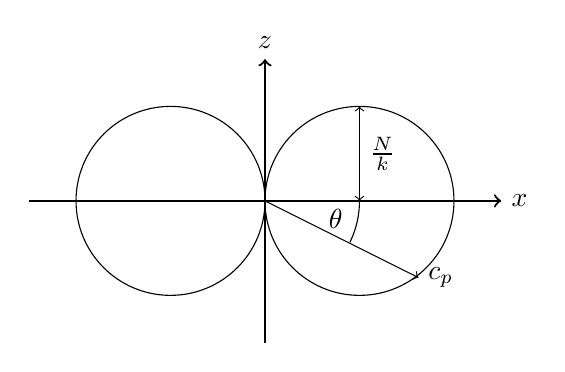
\begin{tikzpicture}[scale=1.5]
		\draw[thick,->] (-2, 0) -- (2, 0) node[right] {$x$};
		\draw[thick,->] (0, -1.2) -- (0, 1.2) node[above] {$z$};
		\draw (0.8, 0) circle (0.8);
		\draw (-0.8, 0) circle (0.8);
		\draw[->] (0,0) -- (1.3, -0.65) node[right] {$\symbf{c}_p$};
		\draw[<->] (0.8, 0) -- (0.8,0.8) node [midway,right] {$\frac{N}{\abs{\symbf{k}}}$};
		\draw (0.8,0) arc (0:-26:0.8);
		\draw (0.6, -0.15) node {$\theta$};
	\end{tikzpicture}
\end{center}

The group velocity is
\begin{equation}
	\symbf{c}_g = \frac{\partial \omega}{\partial \symbf{k}} =
	\frac{1}{2\omega} \frac{\partial \omega^2}{\partial \symbf{k}} =
	\frac{\omega}{\abs{\symbf{k}}^2} \left( \frac{N^2}{\omega^2} K\symbf{k} -
	m \symbf{\hat{z}}) - \symbf{k}\right) = \frac{N}{\abs{\symbf{k}}}
	\abs{\sin\theta} \begin{pmatrix} \cos \varphi \sin \theta \\ \sin \varphi
	\sin \theta \\ -\cos \theta \end{pmatrix}
\end{equation}
Hence the magnitude of the group velocity is $N
\abs{\sin\theta}/\abs{\symbf{k}}$. The group velocity is perpendicular to the
phase velocity:
\begin{center}
	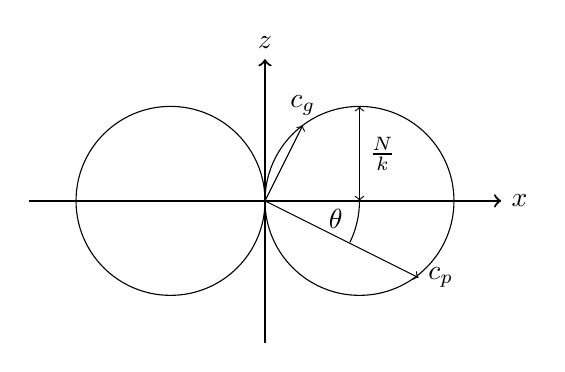
\begin{tikzpicture}[scale=1.5]
		\draw (0.8,0) arc (0:-26:0.8);
		\draw (0.6, -0.15) node {$\theta$};
		\draw[thick,->] (-2, 0) -- (2, 0) node[right] {$x$};
		\draw[thick,->] (0, -1.2) -- (0, 1.2) node[above] {$z$};
		\draw (0.8, 0) circle (0.8);
		\draw (-0.8, 0) circle (0.8);
		\draw[->] (0,0) -- (1.3, -0.65) node[right] {$\symbf{c}_p$};
		\draw[<->] (0.8, 0) -- (0.8,0.8) node [midway,right] {$\frac{N}{\abs{\symbf{k}}}$};
		\draw[->] (0,0) -- (0.32, 0.64) node[above] {$\symbf{c}_g$};
	\end{tikzpicture}
\end{center}

Note that 
\begin{equation}
	\symbf{c}_g + \symbf{c}_p = \frac{N}{\abs{\symbf{k}}} \left[
	\abs{\cos\theta} \begin{pmatrix} \cos\varphi \cos\theta \\
	\sin\varphi\cos\theta \\\sin\theta \end{pmatrix} + \abs{\sin\theta}
	\begin{pmatrix} \cos\varphi\sin\theta\\\sin\varphi\sin\theta \\
	-\cos\theta \end{pmatrix} \right] = \frac{N}{\abs{\symbf{k}}}
	\begin{pmatrix} \cos\varphi \\ \sin \varphi \\ 0 \end{pmatrix}
\end{equation}
Hence $\abs{\symbf{c}_p + \symbf{c}_g} = N/\abs{\symbf{k}}$ and $c_{pz} =
-c_{gz}$. Note also that $\symbf{c}_p \cdot \symbf{c}_g = 0$.

\subsection{Equipartition of energy}
We can form an energy equation from the momentum equation dotted with
$\symbf{u}$:
\begin{equation}
	\symbf{u} \cdot \left( \rho \frac{\partial \symbf{u}}{\partial t} + \rho
	(\symbf{u}\cdot\nabla)\symbf{u} + \nabla p + \rho g \hat{\symbf{z}}\right)
	= 0
\end{equation}
Using the Boussinesq approximation and linearising, we get
\begin{align}
	\symbf{u} \cdot \left( \rho_0 \frac{\partial \symbf{u}}{\partial t} +
	\nabla p' + \rho' g \hat{\symbf{z}}\right) &= 0 \\
	\frac{1}{2}\rho_0 \frac{\partial}{\partial t} \abs{\symbf{u}}^2 +
	\symbf{u} \cdot p' + w \rho' g &= 0
\end{align}
The first term is the rate of change of kinetic energy, the second is the work
against pressure gradients, and the last is the rate of change of potential
energy.

Using linearised conservation of mass we have
\begin{equation}
	\frac{\partial \rho'}{\partial t} + w \frac{\diffd \hat{\rho}}{\diffd z} =
	\frac{\partial \rho'}{\partial t} - w \frac{\rho_0}{g} N^2 = 0 \implies w
	= \frac{g}{\rho_0 N^2} \frac{\partial \rho'}{\partial t}
\end{equation}
Hence also using $\nabla \cdot \symbf{u} = 0$ we have the energy equation
\begin{equation}
	\frac{\partial}{\partial t} \left[ \frac{1}{2}\rho_0 \abs{\symbf{u}}^2 +
	\frac{1}{2}\frac{g^2}{\rho_0 N^2} \rho'^2 \right] + \nabla \cdot (p'
	\symbf{u}) = 0
\end{equation}
The term proportional to $\rho'^2$ is \emph{potential energy}. To see this,
consider a parcel of fluid raised vertically by some amount $\zeta$. The
buoyant force on the parcel is
\begin{equation} 
	F = V g \frac{\diffd \hat{\rho}}{\diffd z} (z-z_0)
\end{equation}
Hence the potential energy gained is
\begin{equation}
	E = \int_{z_0}^{z_0 + \zeta} g \frac{\diffd \hat{\rho}}{\diffd z} (z-z_0)
	\, \diffd z = \frac{1}{2} \rho_0 N^2 \zeta^2
\end{equation}
Using the hydrostatic relation shows that this value matches the potential
energy term in the energy equiation.

\end{document}
